\chapter{Background}
\label{ch:background}

This chapter introduces fundamental concepts and elaborates on the terminology introduced in the previous chapter. This chapter serves to relate practical challenges to research challenges and explains how the two can support each other.

\section{Game Design}
% Game designing is a part of the game development process. Game designers create a theoretical set of mechanics that define a game and game developers implement those mechanics as game software.

Game design is part of the game development process. Game designers create the game on a conceptual level, including declaring a rule-set which becomes the game mechanics. Game developers implement the rule-set as software to provide players with the affordances they define. Game design is an iterative process. Game mechanics evolve as the requirements for the game change, and as such playtesting those mechanics is required even after their final implementation.

The goal behind game design is to create a certain user experience, whether entertainment-based or educational. The user experience that game mechanics create within the context of a game is called gameplay. Gameplay is an elusive concept that researchers have long tried to specifically define\cite{DBLP:conf/digra/ErmiM05}. Crawford\cite{10.5555/538111} broadly defines gameplay as the relation between challenge and player capabilities. In this context, good gameplay is gameplay that seeks to maintain those two notions in balance. Influencing the player's capabilities is complicated but the game designer has complete control over the challenge that the game presents. Game mechanics created by the designers serve to shape that goal. Game mechanics are playtested on whether or not they create that experience. Game designers are already supported by many types of tools and techniques. They can create paper prototypes, rely on player metrics or documentation to judge the impact of mechanics before implementation. 

% Explain what things affect gameplay quality and how they affect them
The quality of the game depends on many different factors. These factors include the visual look of the game, its narrative, the performance, and the one that interests us, the game mechanics. Validating the mechanics is done by playtesting. Playtesting can be conducted manually by humans or by AI agents and it can be conducted before or after the mechanics are implemented with the use of techniques like paper prototypes.\cite{10.1201/b22309}

Playtesting with AI agents is a more recent innovation that aims to make playtesting faster and more reliable\cite{DBLP:journals/corr/abs-1903-10545}. However, it presents its own set of challenges. As an AI-agent learns much more slowly than a human player since human players can draw on their previous experiences, whereas AI agents usually start from zero. Additionally, while AI can test the mechanics in complex ways, they do not experience them the same way that human players do. In this thesis, we focus specifically on addressing the issues caused by human playtesting. AI-based playtesting has its own set of issues and benefits that fall out of the scope of this project. A workshop study by the HCI Institute\cite{10.1145/2967934.2968103} has found that student game developers struggled to integrate the playtesting phase within the iterative design process. Instead, the students would frequently leave playtesting to be closer to the release date, often revealing flaws too late. Similar issues occur within the industry where playtesting reveals major issues with certain game mechanics but due to time constraints, the game is released anyways. 

Game mechanics interact with each other in various ways, they can complement, oppose, be neutral, be pre-requisite and many other ways. Making sure that mechanics interact in the right way is a question of trade-off. When game designers evolve game mechanics to make them more interesting this usually comes at the cost of opposing game mechanics while complementary mechanics also become indirectly more interesting. Making sure game mechanics exist in an equilibrium is called \emph{balancing}. Balancing game mechanics is a complex part of the process that involves a lot more than just changing mathematical values. The aim of that process is ensuring that different strategies remain competitive even as the rules change and as a result, creating the experience the game designer desires. Schell\cite{schell2008art} identifies 13 criteria that contribute to game mechanic balance. These criteria focus on creating an interesting and entertaining experience by balancing challenges and rewards. 

Playtesting validates these criteria, but we aim to provide a solution that can provide rapid feedback and as such, we need a quick way to check if a game mechanic meets some of these criteria. To achieve this we reverse the problem, instead of checking if a game matches any of these criteria, we instead focus on checking if any of the game mechanics really go against the criteria. For example, one way to check if a game mechanic is interesting is to solve a level that makes use of it, either manually or using an AI player. This is time-consuming, so instead, we check to see if the game mechanic does not accidentally create an uninteresting solution such as being able to resolve the challenge by walking in a single direction. We seek to identify other such uninteresting solutions and make it possible to conduct these analysis automatically without the intervention of human playtesters.

\section{Automated Game Design}
% Automated game design (AGD) is a research area that studies how software can help in automatically designing or redesigning games. The aim is to speed up and improve iterative game design processes by automating them. 

Automated game design (AGD) is a research area that studies how software automation can help in speeding up and improving iterative game design. AGD shifts the designer's efforts away from error-prone and repetitive tasks. This allows designers to focus on the creative aspect of the process and explore the design space of their game. AGD is often researched from an AI perspective, which means a focus on the development and application of algorithms. We discuss this perspective but our thesis remains focused on AGD from a meta-programming perspective. The meta-programming perspective is a focus on the engineering of user tools for code analysis and transformation. Procedural content generation (PCG) is defined as \textit{the algorithmic creation of game content with limited or indirect user input}\cite{proceduraltogelius2011}. The content in this case is anything that is contained within the game: levels, rules, entities, sounds, sprites, etc. This definition does not include any of the technical sides of the game such as the engine or the source code. Specifically for this thesis, we are interested in \textit{'interaction-bound content'}, content that affects how the player interacts with the game. 

Interaction-bound content in the context of PuzzleScript is Objects, Rules, Win Conditions and Levels. This can be summarized as the content that affects the player interactions, also referred to as game mechanics. We make this distinction as opposed to other content such as visuals, sounds, or narrative which do not directly contribute to the interactivity of the game. This is not to say that these elements do not contribute to the quality of the game but simply that it is not in the scope of this thesis to understand how audio-visual content impacts game design. In this thesis, we focus specifically on the rules of a game. Rules provide the player with affordances such as walking, jumping, teleporting, or the ability to push other objects. This is similar to moving a piece in chess or playing a card in Uno, what rules allow players to do differ from game to game. Representing rules as content enables us to change the player experience. Rules can be modified manually by a designer or automatically using a tool that embeds an algorithm.

Game quality is limited by the number of design iterations, producing high-quality games requires a reduction of the iteration time. Overcoming that limitation is an important objective of AGD. We can leverage live programming to provide live (immediate and continous) feedback on the quality of game mechanics to achieve this goal. Live programming provides game designers with feedback without the need for an independent testing phase. There are no 'breaks' in the designing process, only minor adjustments\cite{10.1145/3412843}. However, the best way to validate the user experience is still playtesting, so instead of trying to replace playtesters, we simply apply AGD theory to reduce their workload allowing more focus on the complex parts of playtesting.

PCG is not the focus of this thesis but an important part of AGD research and as such, we felt it was necessary to touch on the matter. This thesis focuses more on the use of AGD for automated playtesting, which is more commonly done through the use of AI agents. PCG tools address different challenges based on what they seek to generate. PCG tools aim to generate new levels to leverage existing game mechanics to create an interesting player experience, while others seek to generate the game mechanics themselves. PCG usually requires a level of user input, when the tool and the designer take turns modifying the rules it is called \emph{'mixed-initiative'} design\cite{DBLP:conf/chi/Smith14}. The designer provides settings or inputs that are interpreted by the tool to generate parts of the game, the designer can then adjust the setting or modify the generated content. Mixed-initiative design tools help designers generate much more specific game content that is more in line with their goals without needing to be trained like an AI. 

% Using PCG can drastically speed up the design process of whatever is being generated. 

Using automation such as PCG can have large benefits on the productivity but automation also has a cost. This is especially important as the number of person-months that it takes to create a successful commercial game has increased consistently\cite{shaker2016procedural}. As such, game designers are seeking to speed up part through the use of PCG. This can mean a significant reduction in the cost of game development, making it much easier for smaller teams of developers to hit the "successful" milestone. However, automation has a cost, as automation systems become more complex, game designers begin to get pushed out of the game development process.

PCG is a set of techniques that can aid in the development of interesting games but it can also be integrated directly into the game to generate procedural content even as the game is being played. Games leverage PCG to generate randomized levels that greatly increase the replay value of the game. For the player, it means that no two playthroughs are the same even if they may be more or less similar depending on the complexity of the generator. One of the most famous games to use PCG in that way is Minecraft\footnote{\url{https://www.minecraft.net/}}, an open-world sandbox. Minecraft generates a world in which the player interacts procedurally, placing rivers, forests, mountains, and caves using a complex algorithm. Such types of PCG usually require a small amount of user input to ensure true randomness in their generation.

Studying automated game design is a complex task. Game are huge projects with many components. To study automated game design, we need a concrete problem that is simple enough to study but still fulfills the technical requirements of a game engine. We select PuzzleScript and explain our reasoning in the next section.

\section{PuzzleScript}
Next, we give a limited overview of related work on PuzzleScript that clarifies what is missing in the state of the art for answering our research questions. PuzzleScript is a tiny online online game engine that was identified in a mapping study by van Rozen\cite{10.1145/3412843}.

PuzzleScript is an open-source HTML5 puzzle game engine written using JavaScript by Stephen Lavelle. A PuzzleScript game is made up of 5x5 sprites called Objects, which are used to construct tilemaps called Levels. The player uses the affordances provided by the game mechanics to alter the level with the goal of fulfilling an arbitrary victory condition. Game mechanics are defined using patterns that match a level horizontally or vertically called Rules. If a pattern matches, a replacement pattern is applied, transforming the level.

\begin{figure}[!t]
    \centering
    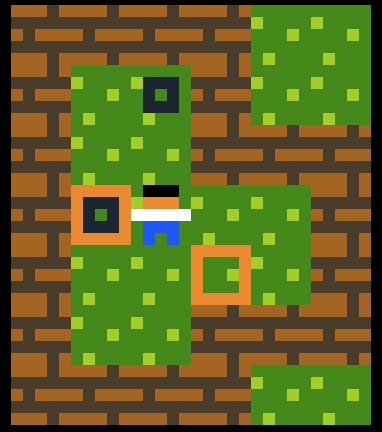
\includegraphics[width=0.40\textwidth]{images/sokoban.png}
    \caption{A simple PuzzleScript game}
    \label{fig:simple_game}
\end{figure}

PuzzleScript closely relates game design and game development through its Rule system. Many game mechanics in PuzzleScript games are literally defined with a single line. This makes it considerably easier to understand how alterations in the game code can affect game mechanics and gameplay. Such an example can be seen in Figure \ref{fig:push_mechanic} where a single line allows the player to push an entity in any direction. Reversing the arrow would allow the player to pull the entity, the entity can also be a reference to multiple entities allowing for a single line of code to affect multiple interactions. 

\begin{figure}
    \centering
    \begin{lstlisting}[language=PuzzleScript]
        [ $\color{violet}>$  Player | Crate ] $\color{BurntRed}->$ [  $\color{violet}>$  Player | $\color{violet}>$ Crate  ]
    \end{lstlisting}
    \caption{Code for push mechanics}
    \label{fig:push_mechanic}
\end{figure}

At its core, this rule system is a simple match and replace pattern. The designer defines a pattern on the left side that is either matched horizontally or vertically and then replaced with the pattern on the right side. In Figure \ref{fig:push_mechanic}, the patterns can be translated to "if a player tries to move into an adjacent crate, then move both entities in that direction". This simple core makes PuzzleScript very approachable by game designers of all levels and its flexibility still allows them to make relatively complex games. One of the contributions from the bachelor thesis by Vermeulen\cite{vermeulenautomated} is a prototype grammar to parse PuzzleScript. This provides support for generating code based on desired player affordances. The prototype parses a significant amount of PuzzleScript rules and serves as the foundation for our own grammar. As a prototype, it fulfills the role of parsing simple PuzzleScript games but it is not a complete grammar. Many of the finer details and corner cases of PuzzleScript's grammar are missing. We use the grammar and design formalization presented in the thesis as a stepping stone.

% Originally written in Dutch, a translator allowed us to make use of their work on reverse engineering PuzzleScript's grammar and of their prototype to get started.

% Several journals and personal accounts\cite{osborn2015playspecs}\cite{8901975}\cite{10.1145/2908812.2908920}\cite{6932896} help us understand PuzzleScript's popularity as a puzzle game engine and its appeal as a language for researching game design.

PuzzleScript's popularity as a game engine and its appeal as a case for researching game design is shown in several papers\cite{osborn2015playspecs}\cite{8901975}\cite{10.1145/2908812.2908920}\cite{6932896}. The papers provide a proof of PuzzleScript's popularity as a game engine with raw statistics and provide motivation arguments for its use within an automated game design perspective. The papers also discuss procedural content generation within PuzzleScript. The common thread between all these papers is that they demonstrate how the concepts we touch one can be used within PuzzleScript and how PuzzleScript is a legitimate case for realistic game research. In addition to Vermeulen's thesis, we also found other papers with interest in Procedural Content Generation. A paper by Krishnan\cite{krishnan2018level} is an example of people studying PuzzleScript games to research game design.

% During our research, we came across several prototypes that aimed to

Several projects that seek to extend or reimplement PuzzleScript in a different language already exist. They provided insights into the processes of the original JavaScript implementation and as such we felt it was important to give a brief overview. The PuzzleScript repository has 127 forks\footnote{\url{https://github.com/increpare/PuzzleScript/network/members}} at the time of writing, of those only a few are actively developed as extensions to PuzzleScript, the rest are either inactive or developed with the intent to merge back into the original with a pull request.

Pattern-Script\cite{PatternScript} is a major extension of the original PuzzleScript engine by Clement Sparrow. It aims to add a plethora of new features\footnote{\url{https://github.com/ClementSparrow/Pattern-Script/wiki}} and support for game designers. By providing additional keywords, the engine allows designers to use shortcuts for the creation of tilemaps and grants them a more granular control on the rule matching process. The extension does not modify the engine and does not extend the behavior of rules, instead it allows designers to restrict the conditions of the rules more tightly. This seems to go along our theory that extending PuzzleScript is hard because the engine's complexity.

This fork by Joe Osborn\cite{PuzzleScriptGA} claims to integrate game analysis but does not seem to have got any commits since the fork was made. Another example is the fork by Rikki Prince\cite{PuzzleScriptTracery} that attempts to make it possible to generate PuzzleScript games using grammar but does not provide working instructions. 

The implementations we found have similar goals to our own. However, unlike our approach, these implementations are all ports of the original PuzzleScript implementation with minor changes. We instead create a complete redesign of PuzzleScript that permits us to create algorithms and tools that can analyze its structure and semantic. This redesign is necessary for answering our research question and the reason we cannot use existing implementations for this project.

\begin{itemize}
    \item C\cite{puzzleengine}: Released, runs simple games.
    \item Rust\cite{puzzlescriptrust}: Released, feature-complete as far as we are aware, needs games to be formatted in a special JSON-based structure
    \item C++\cite{Psionic}: Released, missing features
\end{itemize}

Re-implementations provide insight into how other languages solve the technical complexity of PuzzleScript's rule system. The ones studied here all follow a similar approach to the original JavaScript implementation: hand-crafted parsers that statically check the game at the same time and tightly coupled phases.

Finally, we have works that extend the PuzzleScript implementation in small ways\cite{smoothscreen}\cite{irreversible}. These forks are usually created by programming-inclined PuzzleScript game designers, which have a specific need that the current implementation does not meet. The additions and modifications they perform provide insight into the needs of PuzzleScript developers and designers.

\section{Meta-programming}
Meta-programming is a programming technique that creates \emph{meta-programs}. Normal programs process and transform data, meta-programs process and transform other programs. Meta-programming techniques and language workbenches help programmers in the activities of meta-programming. Domain specific languages (DSL) are programming languages that perform a very specific set of tasks, compared to general-purpose languages which can be used for a wide range of tasks. PuzzleScript is an external DSL with the specific purpose of creating top-down or 2D puzzle games. One would be unable to use PuzzleScript to create websites or calculate financial data, that is outside the domain.

PuzzleScript makes use of meta-programming in its JavaScript implementation to transform rules into JavaScript functions. In this scenario, we see one of the limitations of this specific brand of meta-programming: code obfuscation. A significant part of the code that processes rules of a PuzzleScript game does not exist before runtime, this makes it much harder to maintain and extend. This decision hurts the readability and searchability of the codebase in that a programmer must first compile a game before being able to observe how the rules transform into code. Only having that complete overview during runtime makes it harder for programmers to identify and locate bugs.

Language workbenches can help to facilitate meta-programming. We use Rascal, a meta-programming language and language workbench to parse, run and analyze PuzzleScript games. We selected Rascal from a list of meta-programming languages and language workbenches identified by van Rozen\cite{10.1145/3412843} and in a paper on language workbenches for game development\cite{10.1007/978-3-319-02654-1_3}. Domain-specific languages have been successfully applied in many domains but their benefits to game development are not yet clear. According to this paper by Klint and van Rozen\cite{10.1007/978-3-319-02654-1_3}, this is due to the game domain being very diffuse. It is hard to analyze a moving domain where modeling and software reused are limited. The existing approach is game engines which provide the ability for software reuse and optimization, but even these have very specific cases and no silver bullet exists.

In this thesis on the state of the art in workbenches, several other language workbenches are identified. It also identifies several features deemed essential in language workbenches and compares the identified list with the workbenches themselves. From that, we can see Rascal is not the most feature-complete of the workbenches presented, but it provides the ability to make up that difference programmatically. 

Rascal is an extensible meta-programming language and IDE for source code analysis and transformation with the goal to merge the SCAM (source code analysis and manipulation) domain into a single language\cite{Klint2011}. It provides parsing in the form of its Syntax Definition Formalism that allows developers to create a literal representation of the programs they are trying to parse through the use of lexical and symbols. These representations can then be converted by \textit{imploding} them into equivalent data structures. Rascal also offers the possibility of processing concrete syntax which does not require implosion but has other downsides. Rascal also implements the concept of \textit{visiting}, which allows us to traverse an arbitrarily complex subject and apply a number of cases to all its nodes. We can use this to enrich a parse tree without having to modify its structure by editing or replacing individual nodes.


Finally, Rascal presents a concept called "Abstract Patterns" which allows us to match data structures using regular patterns similar to how one might match text with regular expressions. This concept is very similar to the way that PuzzleScript Rules work on the surface and as such we believe that it is possible to use it to create a more human-readable version of compiled Rules. In the current implementation, Rules are compiled into functions, which adds a layer of complexity as part of the codebase that can only be observed during runtime.  

\section{Reverse Engineering}
Our project aims to create a version of PuzzleScript that is well suited for game design research, extension and maintainability. Unfortunately, we cannot simply port the existing JavaScript implementation. We need access to PuzzleScript's design to create our own implementation. Since the design of PuzzleScript is not fully documented, we have to reverse engineer the existing implementation.

Reverse engineering is the method of attempting to understand how a program works by deductive guesses based on the observation of the program's behaviors\cite{10.1145/336512.336526}. Researchers who reverse engineer programs do not always have access to the full source code or architecture documents and as such must rely on their observations to guess the original intentions of the developers. There are two main aspects to reverse engineering: redocumentation and design recovery. Redocumentation is the process of creating a new representation of a program and design recovery is the process of using deduction in relation to one's experience with the product to recover its design\cite{43044}.

Reverse engineering is commonly used in cases where the source code is inaccessible, however, that is not a requirement. Reverse engineering can also be used when the source code is not properly documented or densely structured to reconstruct the design of the application. This method is not without flaws, it requires a good understanding of the language the program is written in. Knowledge gaps can sometimes be filled by observing the behavior of the application from the user perspective. Reverse engineering is very time consuming, but it is sometimes the only option to be able to separate the design from the implementation.

The process of design recovery involves connecting the codebase to user-facing endpoints to understand how they fit together. Observing the behavior of a program is a relatively safe way of ensuring that the correct intent is understood, but it depends heavily on managing to trigger every corner case. Complementing this is the method of going through the codebase\cite{10.5555/2555229}. This method presents its own set of issues depending on how strict the language is with its typing. 

The end product of design recovery is a design document based on the observed behaviors. This document is made up of assumptions the person conducting the reverse engineering made therefore it is not a pure version of the original design. Purifying that version to be closer to the original is a task that requires a lot of work but can be supported by specialized techniques such as model-based reverse engineering\cite{DBLP:journals/computer/Biggerstaff89}.

